\section{Introduction}\label{sec:introduction}

A relaxed control can divide activity among several operating modes, whereas
an implementable switching control activates one mode at a time. Combinatorial
integral approximation measures the resulting discrepancy by the largest
absolute difference between cumulative mode allocations. A fine grid permits
small discrepancy when switches are unrestricted. With a hard switch budget,
refining the grid only improves the placement of finitely many changes; it
cannot remove the approximation error caused by the budget itself. The
relevant questions are therefore quantitative: what error is unavoidable,
which relaxed inputs attain it, and how can one compute an optimal or
certifiably near-optimal schedule?

We answer these questions for measurable simplex-valued controls on a horizon
$[0,T]$, with $n$ modes and at most $s$ switches. The initial mode is free,
repeated modes are allowed, and the default model has no dwell or transition
restrictions. For an input cumulative allocation $A$, write $\OPT_s(A)$ for
the smallest cumulative discrepancy among continuous-time schedules and
$F_{n,s}(T)=\max_A\OPT_s(A)$ for its worst-case value. A superscript
$\mathcal T$ restricts switching times to a specified grid. The distinction
between an input optimum and the maximum over inputs is essential: a sharp
bound on the discretization error of each input does not establish a sharp
gap between two worst-case values.

\subsection{Results and proof strategy}

Our main continuous minimax formula is
\begin{equation}\label{eq:intro-main}
 F_{n,s}(T)=T\max\left\{\frac{1}{s+2},
 \frac{1}{n\bigl((n/(n-1))^{s+1}-1\bigr)}\right\},
 \qquad 0\le s\le3,\quad n\ge s+2.
\end{equation}
A uniform input supported on $s+2$ modes attains the first term. The second
is the sharp one-sided error for the uniform input on all $n$ modes. This
geometric term exceeds the plateau term starting at $n=5,8,12$ for
$s=1,2,3$, respectively. Figure~\ref{fig:minimax-regimes} illustrates these
transitions. The formula includes all measurable inputs, and its lower proof
allows competing schedules to repeat modes.

\begin{figure}[tb]
\centering
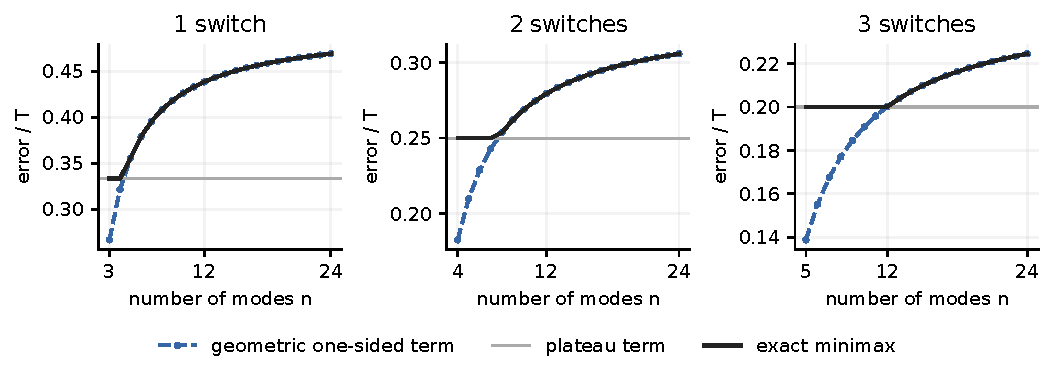
\includegraphics[width=\linewidth]{figures/minimax-regimes.pdf}
\caption{The exact continuous minimax value divided by $T$, its plateau term, and
the geometric one-sided uniform term
for one, two, and three switches, on their stated mode ranges. Lines connect
integer mode counts.}
\label{fig:minimax-regimes}
\end{figure}

The main reduction separates a heavy-mode case from a one-sided discrepancy
problem. If some terminal mode mass exceeds $E$ and $T\le(s+2)E$, an integral-prefix rounding and a reordering of the first repetition produce an
$s$-switch schedule of full error at most $E$. Otherwise, a one-sided bound
suffices. We prove sharp reach bounds using distinct modes through four
blocks. The two- and three-block arguments are analytic. The four-block
argument uses an explicitly defined necessary-condition linear program,
exhaustive symmetry reduction, and exact rational and polynomial dual
certificates covering every $n\ge5$. Floating-point optimization is not a
proof dependency. At the boundary $n=k=3$, a constructed input has an exact
three-block one-sided optimum strictly worse than the uniform input, even
when repeated modes are allowed. Thus the spare-mode hypothesis in this
reach method has mathematical content.

For arbitrary block count $k=s+1<n$, removing either a largest-mass or a
smallest-mass mode propagates existing bounds. The resulting closed formula
and its four-block seeded improvement yield exact plateau ranges and
\[
 F_{n,k-1}(T)=\frac{T}{k}-\frac{(k+1)T}{2kn}
                  +O_k(Tn^{-2})\qquad(n\to\infty).
\]
The leading dimension-free bound follows from classical integral-prefix
rounding; the first mode-count correction is sharp. Equal-terminal-mass
inputs have additional guarantees, including an exact instance value in a
band next to $n=k$. The remaining general five-block reach question is
isolated in Appendix~\ref{sec:higher-reach}: an earlier event relaxation admits
a nonphysical counterexample, whereas a fully ordered chamber has a matching
exact certificate. Neither observation is used as a proof for other chambers.

On finite grids, a separate extremal analysis gives an explicit one-switch
minimax formula on every rational grid for $n\ge3$, evaluable in $O(N^2)$
rational operations, with a worst input having two component types and at most
three time phases. Three-mode unit grids admit a finite floor-history
representation valid for every length. It gives exact values on five, six,
and seven cells, including $F^{\mathrm{unit}}_{3,3}(7)=4/3$. Its five-cell
consequence closes the continuous boundary value $F_{3,2}(T)=T/5$.
For three modes and three switches, the proved continuous range is
$T/7\le F_{3,3}(T)\le T/6$; an exact value is not asserted.
These results both sharpen and correct specific finite-grid claims in
\citet{sager-zeile2021}. The source comparisons distinguish a false equality,
an upper bound that fails, and a lower bound that fails.

The algorithmic results solve supplied inputs. One-switch optimization takes
$O(nN)$ arithmetic operations on an arbitrary grid. For a fixed number $k$
of nominal blocks, a subset-partition dynamic program assigns blocks to
modes, allowing repeats and checking specified minimum dwell times on maximal
runs. Enumerating the block boundaries gives polynomial time for every fixed
switch budget, with linear dependence on $n$ in the arithmetic bound.
A supported chronological grid transfer preserves the switch budget and
changes cumulative occupations by strictly less than one uniform cell width
$h$. Its coefficient one is sharp uniformly over modes and budgets. Combining
this transfer with exact coarse optimization yields a computable additive
certificate for the continuous optimum, with explicit input-quantization
bounds. Dwell restrictions require separate treatment: an elementary example
has a fixed positive grid gap on arbitrarily fine odd grids.

\begin{table}[tb]
\centering\small
\caption{Main scopes. Here $k=s+1$, and a unit grid has horizon $N$.}
\label{tab:results-synopsis}
\begin{tabular}{@{}p{.32\linewidth}p{.43\linewidth}p{.18\linewidth}@{}}
\toprule
Problem & Result & Reference\\
\midrule
Continuous minimax, $0\le s\le3$, $n\ge s+2$
 & Exact formula~\eqref{eq:intro-main} & Theorem~\ref{thm:small-full}\\
General budgets, $n>k$ & Closed and seeded upper bounds; sharp first correction
 & Section~\ref{sec:general-budgets}\\
Three-mode boundaries & $F_{3,2}=T/5$; $T/7\le F_{3,3}\le T/6$
 & Section~\ref{sec:floor-chambers}\\
One-switch grid minimax, $n\ge3$ & Explicit formula on arbitrary grids
 & Theorem~\ref{thm:finite-one}\\
Three-mode unit grids & $(N,s)=(5,2),(6,3),(7,3)$: values $1,1,4/3$
 & Section~\ref{sec:floor-chambers}\\
Supplied grid input & Exact one-switch and fixed-budget algorithms
 & Section~\ref{sec:algorithms}\\
Continuous-to-grid transfer & Sharp uniform coefficient; additive certificates
 & Section~\ref{sec:transfer}\\
\bottomrule
\end{tabular}
\end{table}

\subsection{Relation to earlier work}

The CIA decomposition and switch-constrained approximation subproblem were
introduced by Sager, Jung, and Kirches~\cite{sager2011cia}, including a mixed
integer linear formulation and a tailored branch-and-bound algorithm.
Sager and Zeile~\cite{sager-zeile2021} study a total-variation constraint on the
integer control and derive worst-case bounds and maximum dwell rounding.
Their multi-mode conjecture is the closest direct comparison for the minimax
results here. The continuous lower constructions and the precise published
finite-grid statements are credited where they are used or corrected; see
Sections~\ref{sec:one-switch} and~\ref{sec:floor-chambers}.

Integral flow and matching are established tools for rounding partial sums;
Knuth's two-way rounding theorem~\cite{knuth1995} is a classical example.
Bestehorn and Kirches~\cite[Corollary~2.7]{bestehorn2021vanishing} prove
support-preserving CIA rounding with discrepancy at most one uniform grid
width. Our transfer proof gives this construction explicitly and adds the
chronological argument that preserves a supplied schedule's switch count,
the strict bound, and a sharp instance-wise discretization family. The
half-grid motivation preceding the conjecture in
\cite[p.~615]{sager-zeile2021} and \cite[p.~139]{zeile2021thesis} is already a
proposed discretization comparison; it is not a proved universal theorem.
Section~\ref{sec:transfer} identifies its valid special cases and an explicit
counterexample to its unrestricted instance-wise interpretation.

Exact graph algorithms for switching costs, minimum dwell times, and support
restrictions already exist. In particular, the shortest-path formulation of
Bestehorn, Hansknecht, Kirches, and Manns~\cite{bestehorn2021shortest} gives
switching-cost-aware rounding (SCARP), with a complexity bound exponential in
the mode count. Zeile, Robuschi, and Sager~\cite{zeile2021dwell} analyze minimum
dwell rounding, and switching-time enumeration is discussed in
\cite[Section~6.4.3]{zeile2021thesis}. More recently,
Abbasi-Esfeden, Plate, Sager, and Swevers~\cite{abbasi2025} propose a flexible
dynamic-programming-inspired CIA method with dwell constraints; their
introduction explicitly states that it does not generally guarantee global
optimality because optimal substructure is lost. The distinction in the
present exact algorithms is the CIA-specific dominance and subset reduction,
with its proved dependence on the mode count for a fixed small budget.
Dynamic programming and dwell-constrained rounding themselves are established.

Several approximation results concern grids whose refinement permits the
number of switches to grow. Tight sum-up-rounding bounds
\cite{kirches2020tight}, compactness and convergence of CIA decompositions
\cite{kirches2021compact}, and adaptive nonuniform refinement for SCARP
\cite{bestehorn2023adaptive} provide this broader setting. Our coarsening
certificate concerns the best approximation with a fixed switch budget and
a prescribed additive accuracy, including exact integration across nonaligned
input and output grids. It does not assert convergence to the relaxed control
at fixed budget. Finally, cumulative discrepancy can bound state error under
appropriate regularity assumptions, as in
\cite[Theorem~1 and Corollary~1]{zeile2022decomposition}. Here the proved and
measured quantities are discrepancy, switching feasibility, and optimization
cost. Claims about nonlinear state constraints, economic objectives, or
closed-loop stability require the corresponding dynamics and assumptions.

\subsection{Organization}

Section~\ref{sec:foundations} gives the model and attainment and stability
properties. Sections~\ref{sec:one-switch}--\ref{sec:small-minimax} establish
uniform-input formulas and the sharp continuous results. The structural
counterexamples in Section~\ref{sec:structural-limits} delimit the constructions.
Sections~\ref{sec:general-budgets} and~\ref{sec:predecessors} develop general
budgets and retain useful input-dependent bounds. The finite-grid minimax
results follow in Sections~\ref{sec:finite-one} and~\ref{sec:floor-chambers}.
Sections~\ref{sec:algorithms} and~\ref{sec:transfer} give the instance algorithms
and coarsening certificates. Section~\ref{sec:computations} reports reproducible
exact computations. Section~\ref{sec:discussion} identifies the remaining
research questions, with the detailed higher-reach analysis in
Appendix~\ref{sec:higher-reach}.
